\documentclass[aip,jap,reprint]{revtex4-1}

%\documentclass[aps,prl,twocolumn,showpacs,superscriptaddress,groupedaddress]{revtex4-1}  % for review and submission
%\documentclass[aps,preprint,showpacs,superscriptaddress,groupedaddress]{revtex4-1}  % for double-spaced preprint
\usepackage[english]{babel}

\usepackage[ascii]{inputenc}
\usepackage[T2A,T1]{fontenc}
\usepackage{amsmath}
\usepackage{amssymb,amsfonts,textcomp}
\usepackage{array}
\usepackage{supertabular}
\usepackage{hhline}
\usepackage{graphicx}
\makeatletter
\newcommand\arraybslash{\let\\\@arraycr}
\makeatother
\setlength\tabcolsep{1mm}
\renewcommand\arraystretch{1.3}

\usepackage{graphicx}% Include figure files
\usepackage[pdftex,unicode,colorlinks, citecolor=blue,%
filecolor=black, linkcolor=blue, urlcolor=black]{hyperref}
\begin{document}

% \documentclass[11pt]{article}
% \usepackage{makeidx}
% \usepackage{multirow}
% \usepackage{multicol}
% \usepackage[dvipsnames,svgnames,table]{xcolor}
% \usepackage{graphicx}
% \usepackage{epstopdf}
% \usepackage{ulem}
% \usepackage{hyperref}
% \usepackage{amsmath}
% \usepackage{amssymb}
\title{Optical Properties of Core/Shell nanoparticles: comparison of $TiO_{2}/Ag$  and
$Ag/TiO_{2}$ structures}
\author{Volodymyr Lysak}
\affiliation{ITMO University, 49 Kronverskii Ave., St.~Petersburg
  197101, Russian Federation\\}
\author{Konstantin Ladutenko}
\affiliation{ITMO University, 49 Kronverskii Ave., St.~Petersburg
  197101, Russian Federation\\}
\affiliation{Ioffe Physical-Technical Institute of the Russian
  Academy of Sciences,
  26 Polytekhnicheskaya Str., St.~Petersburg 194021, Russian
  Federation}
\date{\today}
\begin{abstract}
  Some abstract
\end{abstract}

\pacs% insert suggested PACS numbers in braces on next line
{ Some PACS numbers}
\maketitle %\maketitle must follow title, authors, abstract and \pacs

Nanotechnology is an area of scientific research due to the high
potential applications in media-recorder, defense-industry, optical and
electronic devices. Semiconductor photocatalysis and
photoelectrochemistry, particularly involving $TiO_2$, is an influential
field that plays an important role on environmental remediation and
energy conversion applications. The striking features of $TiO_2$ including
its high chemical stability in aqueous media, high photoactivity, earth
abundance and environmentally benign nature strongly encourage the use
of this material as a potential electron acceptor in light driven
devices operating under solar radiation [1-4]. 

We used the solution of Maxwell's equations for
spherical particles using Mie theory [5-9]. According to this theory,
we calculate the optical efficiency parameters, used MATLAB software
[10], such as the extinction, absorption and scattering for
nanoparticles at different diameter and shell thickness.

In this study, we focused on the optical properties of Titanium
dioxide/ silver core/shell nanoparticles. For this reason, to compute
the efficiency diagrams (scattering, absorbing and extinction curves).
Since the radius of the particles investigated here is smaller than
the mean free path in the bulk metal, the particle radius has been
taken as the mean free path to calculate the dielectric function of
the particles. The dependence of the complex dielectric function of
metal nanoparticles on size is included by replacing the bulk
relaxation constant in the Lorentz-Drude dielectric function by a
radius $R$ dependent quantity as follows [11,12]:
\begin{widetext}
\begin{align*}
\varepsilon(\omega,R) = \varepsilon_{bulk}(\omega) 
+ \omega^2_p
\left(
  \frac{1}{\omega^2 +{\Gamma}^2_{\infty\phantom{A}}} -
  \frac{1}{\omega^2 +\Gamma(R)^{2}_{\phantom{A}}} 
\right)
+ i \frac{\omega^2_p}{\omega}
\left (
  \frac{\Gamma(R)}{\omega^2+\Gamma(R){^2_{\phantom{A}}}}
  - \frac{\Gamma_\infty}{\omega^2+\Gamma{^{2}_{\infty\phantom{A}}}}
\right) ,\\ 
\varepsilon_{bulk}(\omega) = \varepsilon_\infty 
+ \sum^6_{m=1} \frac{G_m \omega^2_p}{\omega_m^2 - \omega^2 -i \omega
  \Gamma_m} , \qquad
  \Gamma(R) = \Gamma_\infty + A\frac{\nu_{\! _F}}{R}, \qquad
  \Gamma_\infty = \frac{\nu_{\! _F}}{l_\infty}
\end{align*}
\end{widetext}
where $\omega$
is the angular frequency, $\omega_p$
is the plasmon frequency of silver, $G_m$
is the strength of each resonance term, $\omega_m$
is the resonant frequency, $\Gamma_m$
is the damping factor or collision frequency, $\nu_{\! _F}$
is the plasmon frequency, $l_\infty$
is the mean free path in bulk metal, $A$
is a shape-dependent factor and can be taken as 1 for spherical
particles.

Parameter values used in calculation: $\hbar\omega_p = 9.01$~eV;
$G_m = [0.845\ 0.065\ 0.124\ 0.011\ 0.840\ 5.646]$; 
$\hbar\omega_m = [0.000\ 0.816\ 4.481\ 8.185\ 9.083\ 20.29]$~eV;
$\hbar\Gamma_m = [0.048 3.886 0.452 0.065 0.916 2.419]$~eV;
$\nu_{\! _F} = 1.39 \times 10^6$; $l_\infty = 52$~nm.

For $TiO_2$ dispersion Sellmeier relation of dielectric function is
applied: 

$$
\varepsilon_{TiO_2} = 2.8731 + \frac{3.04\lambda^2}{\lambda^2-0.2834^2}
$$

Under quasi-static conditions, the absorption $Q_{abs}$ and scattering $Q_{sca}$
and extinction $Q_{ext}$ efficiency coefficients can be calculated from Mie
scattering theory [13]. We analyze efficiency coefficients, which are
the cross-section value normalized to the geometric cross-section of
nanoparticles. Mie theory predicts about all particles, small or large,
transparent or opaque. Mie theory allows for primary scattering from
the surface of the particle and for the secondary scattering caused by
light refraction within the particle.

The optical properties of $TiO_2/Ag$ nanospheres ($TiO_2$ core) are relative
on the nanospheres diameter. Fig.~\ref{fig:spectra}(a,c,e) shows $Q_{abs}$ diagrams for different
core diameters such as 10, 25 and 50~nm at various shell thickness
(5-40~nm). As core diameter increases, related peaks split one another
at small shell thickness. As shell thickness increases, both peaks come
closer that increases full width at half maximum (FWHM) of
efficiency's diagram. 

\begin{figure}
  \begin{minipage}[h]{0.235\textwidth}
    \begin{flushleft}
      a)
    \end{flushleft}
  \end{minipage}
  \hfill
  \begin{minipage}[h]{0.235\textwidth}
    \begin{flushleft}
      b)
    \end{flushleft}
  \end{minipage}
  \begin{minipage}[h]{0.235\textwidth}
    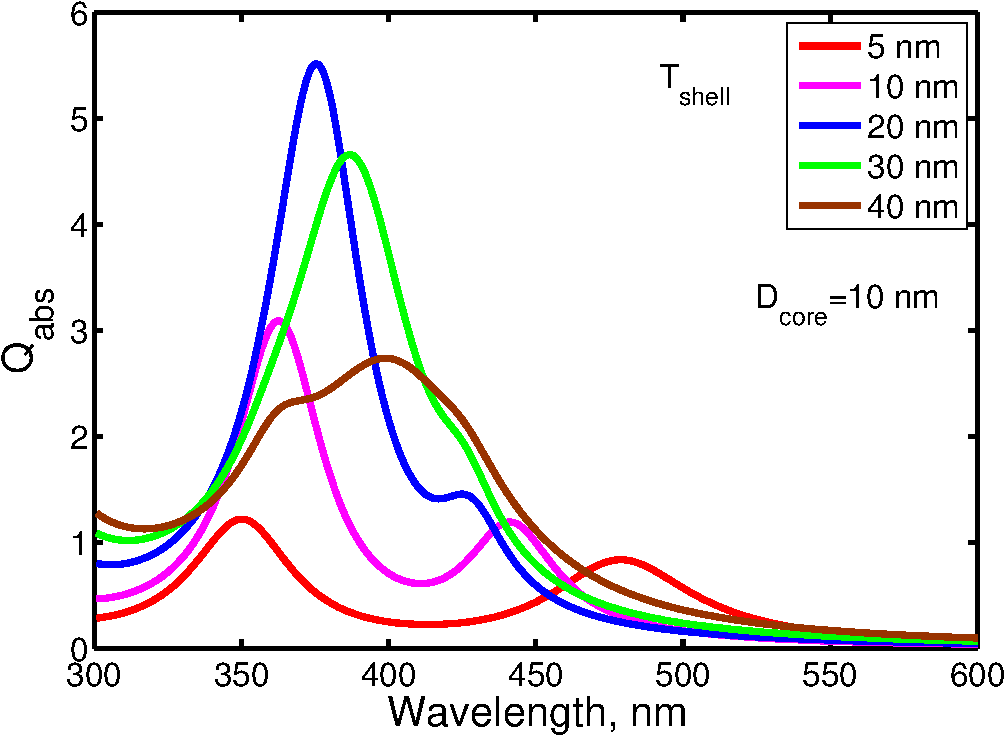
\includegraphics[width=0.99\textwidth]{Qabs_core_10nm}
  \end{minipage}
  \hfill
  \begin{minipage}[h]{0.235\textwidth}
    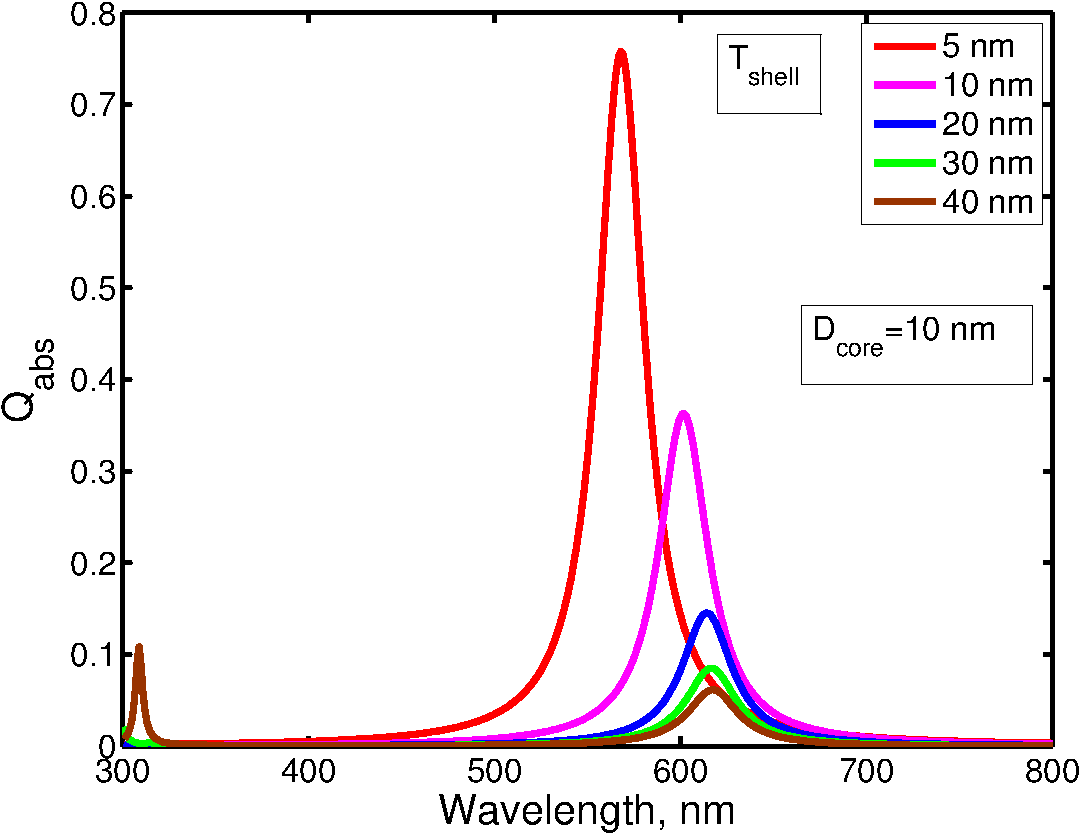
\includegraphics[width=0.99\textwidth]{Qabs_Ag_TiO_10_t}
  \end{minipage}\\
  \vspace{4pt}
  % \vfill
  \begin{minipage}[h]{0.235\textwidth}
    \begin{flushleft}
      c)
    \end{flushleft}
  \end{minipage}
  \hfill
  \begin{minipage}[h]{0.235\textwidth}
    \begin{flushleft}
      d)
    \end{flushleft}
  \end{minipage}
  \begin{minipage}[h]{0.235\textwidth}
    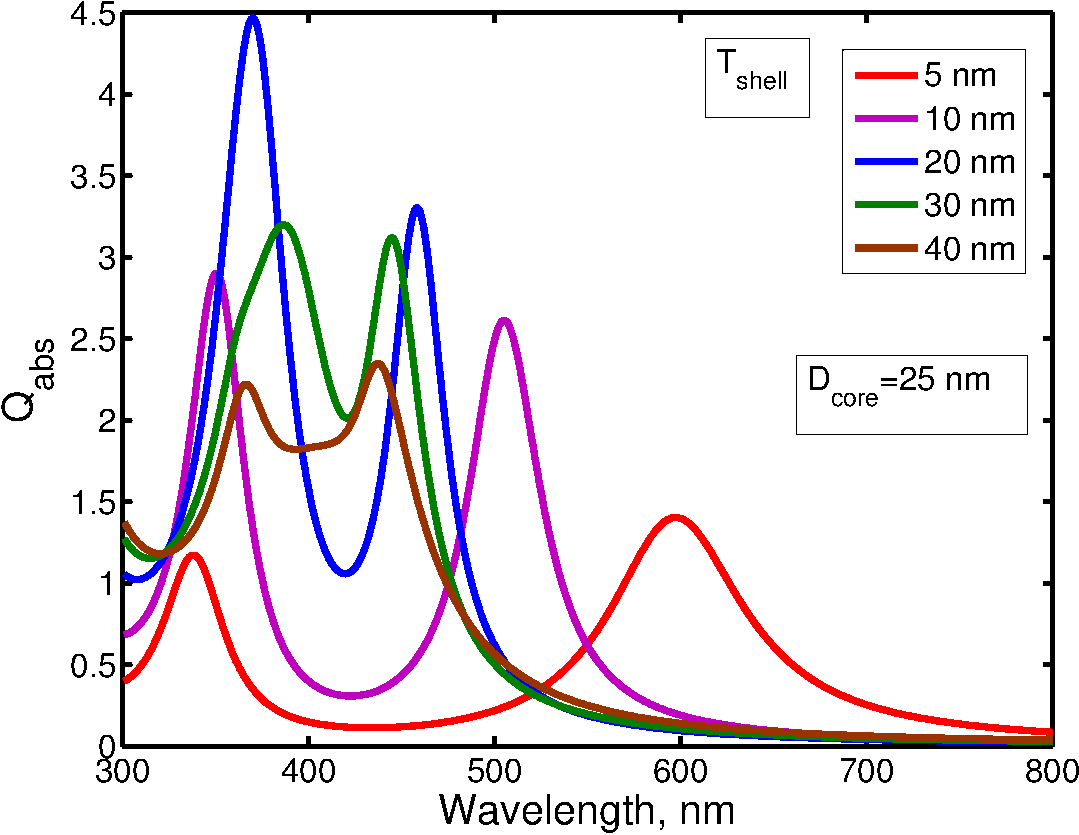
\includegraphics[width=0.99\textwidth]{Qabs_core_25nm}
  \end{minipage}
  \hfill
  \begin{minipage}[h]{0.235\textwidth}
    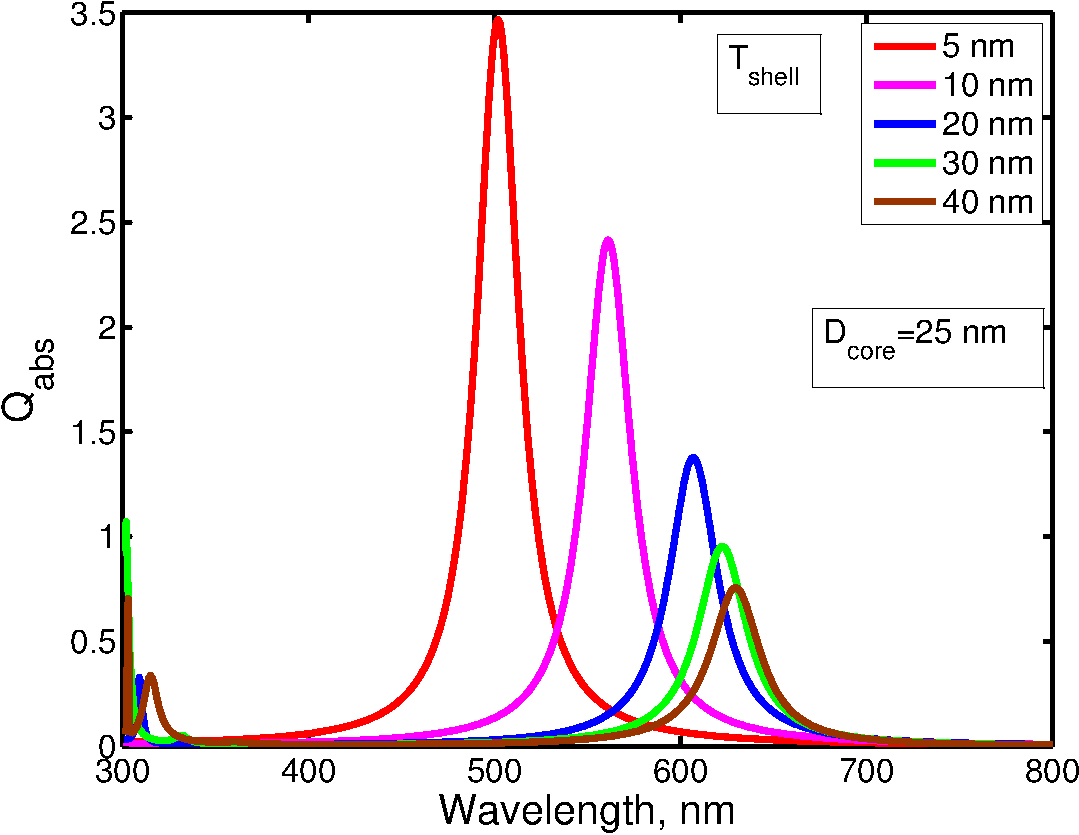
\includegraphics[width=0.99\textwidth]{Qabs_Ag_TiO_25_t}
  \end{minipage}\\
  \vspace{4pt}
  % \vfill
  \begin{minipage}[h]{0.235\textwidth}
    \begin{flushleft}
      e)
    \end{flushleft}
  \end{minipage}
  \hfill
  \begin{minipage}[h]{0.235\textwidth}
    \begin{flushleft}
      f)
    \end{flushleft}
  \end{minipage}
  \begin{minipage}[h]{0.235\textwidth}
    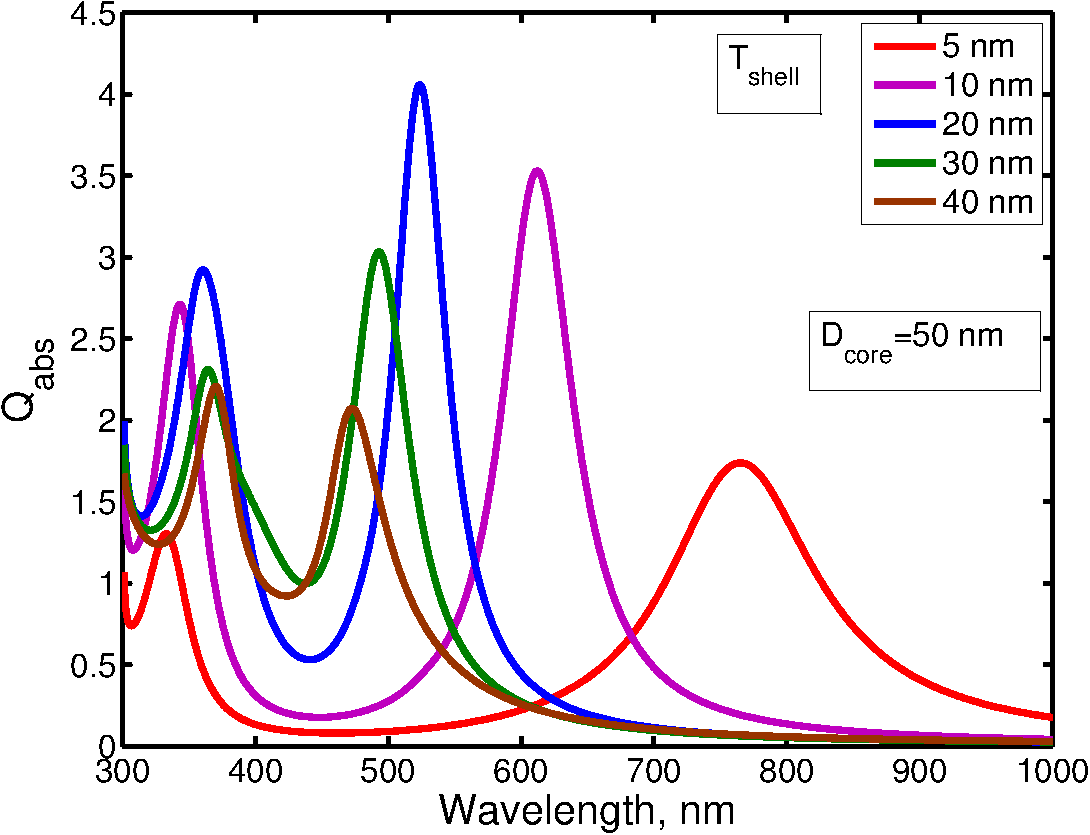
\includegraphics[width=0.99\textwidth]{Qabs_core_50nm}
  \end{minipage}
  \hfill
  \begin{minipage}[h]{0.235\textwidth}
    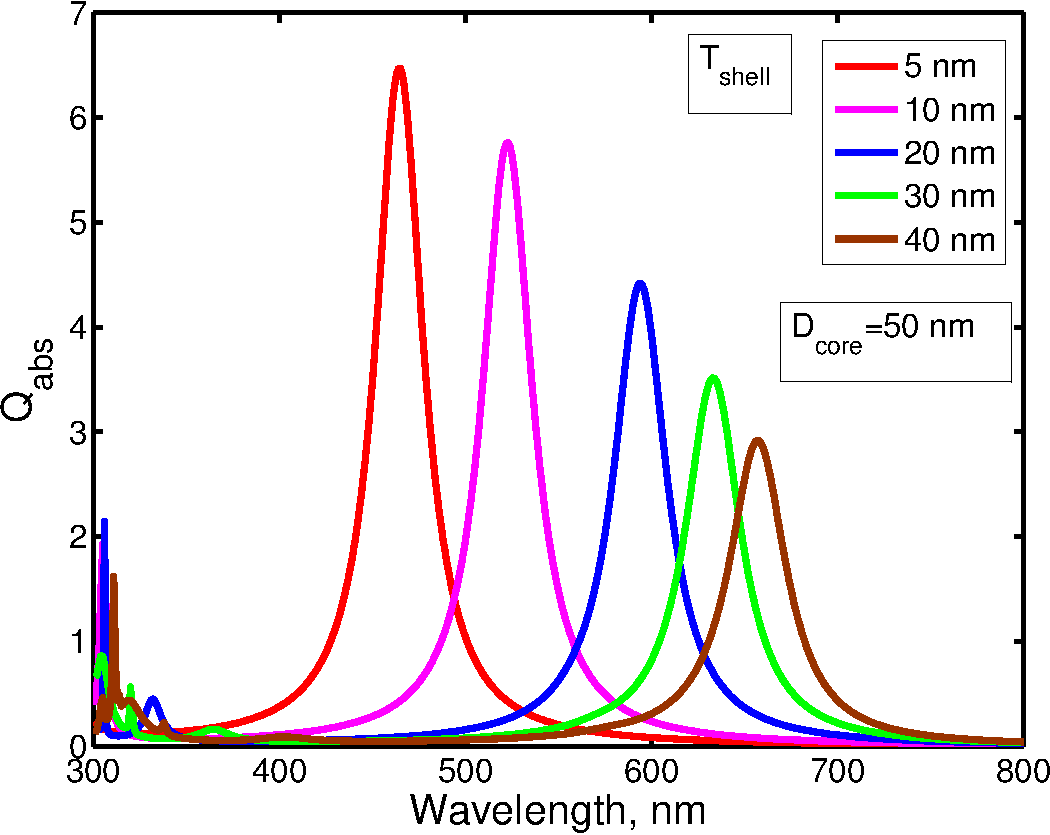
\includegraphics[width=0.99\textwidth]{Qabs_Ag_TiO_50_t}
  \end{minipage}%
  \caption{Absorption spectra for $TiO_2$ (a,c,e) and $Ag$ (b,d,f)
    core with different shell thickness for the core diameter of: (a,b)
    10~nm, (c,d) 25~nm, (e,f) 50~nm.
    \label{fig:spectra}}%
\end{figure}




Fig.~\ref{fig:spectra}(b,d,f) shows similar analysis for $Ag/TiO_2$
core/shell NP (Ag core). In that case, spectra have only one peak
related with silver properties.  Comparison between two structures
shows that oxide/metal NP has lower adsorption efficiency but wider
spectral width, while inverted structure is more efficient with narrow
spectrum.


As an example, the comparison of absorption properties for two
structures is presented. In this case, the thickness of metal shell in
the $TiO_2$ core and the core radius in the Ag core is equal 20~nm.
Thickness of the oxide layer is chosen to overlap absorption peak in
the visible range of spectrum. The core radius of the $TiO_2$ core and
shell thickness of the Ag core is equal to 25~nm and 9~nm,
respectively. Absorption spectra are combined at wavelength of 524~nm
and presented in Fig.~\ref{fig:field}(a) by blue and red line for the $TiO_2$ core and Ag
core, respectively.  As expected, the spectrum of the $TiO_2$ core has
another peak at 360~nm. E/H- field distribution is presented  for the
$TiO_2/Ag$ nanospheres at 360~nm Fig.~\ref{fig:field}(b,c), and at 524~nm for $TiO_2$ core
Fig.~\ref{fig:field}(d,e) and Ag core Fig.~\ref{fig:field}(f,g). The short/long wavelength peak
related to plasmonic interaction on silver-air/$TiO_2$-silver interface,
respectively.
\begin{figure}[!h]
  \begin{minipage}[h]{0.47\textwidth}
    \begin{flushleft}
      a)
    \end{flushleft}
  \end{minipage}
  \begin{minipage}[h]{0.47\textwidth}
    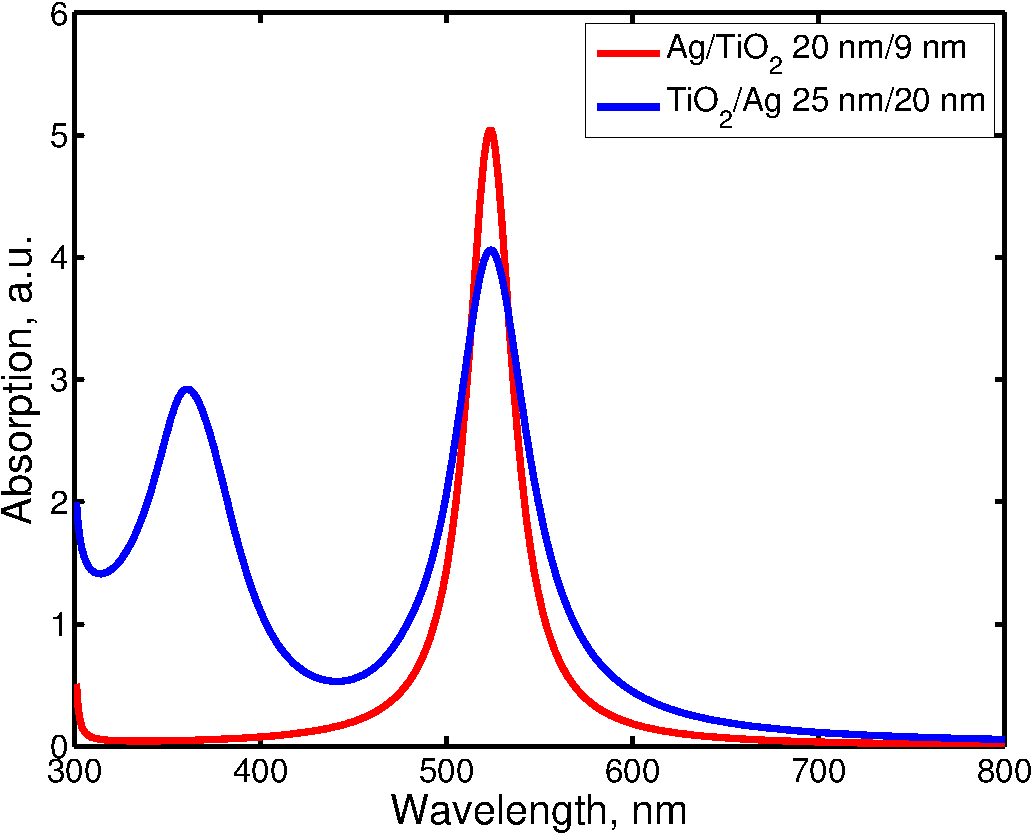
\includegraphics[width=0.99\textwidth]{reverse}
  \end{minipage}\\
  \vspace{4pt}
  % \vfill
  \begin{minipage}[h]{0.235\textwidth}
    \begin{flushleft}
      b)
    \end{flushleft}
  \end{minipage}
  \hfill
  \begin{minipage}[h]{0.235\textwidth}
    \begin{flushleft}
      c)
    \end{flushleft}
  \end{minipage}
  \begin{minipage}[h]{0.235\textwidth}
    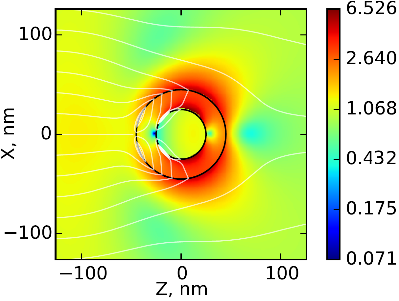
\includegraphics[width=0.99\textwidth]{3b}
  \end{minipage}
  \hfill
  \begin{minipage}[h]{0.235\textwidth}
    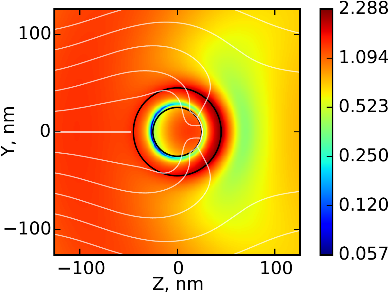
\includegraphics[width=0.99\textwidth]{3c}
  \end{minipage}\\
  \vspace{4pt}
  \begin{minipage}[h]{0.235\textwidth}
    \begin{flushleft}
      d)
    \end{flushleft}
  \end{minipage}
  \hfill
  \begin{minipage}[h]{0.235\textwidth}
    \begin{flushleft}
      e)
    \end{flushleft}
  \end{minipage}
  \begin{minipage}[h]{0.235\textwidth}
    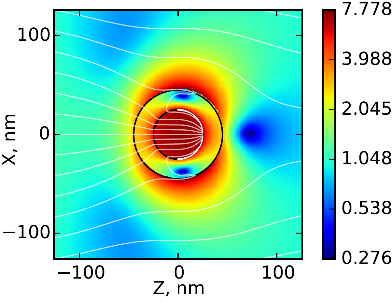
\includegraphics[width=0.99\textwidth]{3d}
  \end{minipage}
  \hfill
  \begin{minipage}[h]{0.235\textwidth}
    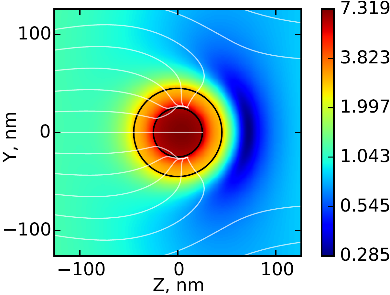
\includegraphics[width=0.99\textwidth]{3e}
  \end{minipage}\\
  \vspace{4pt}
  \begin{minipage}[h]{0.235\textwidth}
    \begin{flushleft}
      f)
    \end{flushleft}
  \end{minipage}
  \hfill
  \begin{minipage}[h]{0.235\textwidth}
    \begin{flushleft}
      g)
    \end{flushleft}
  \end{minipage}
  \begin{minipage}[h]{0.235\textwidth}
    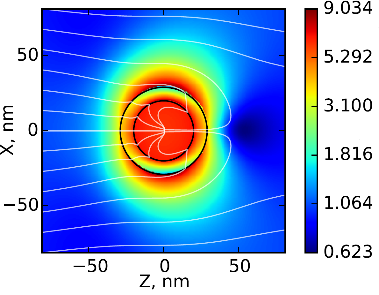
\includegraphics[width=0.99\textwidth]{3f}
  \end{minipage}
  \hfill
  \begin{minipage}[h]{0.235\textwidth}
    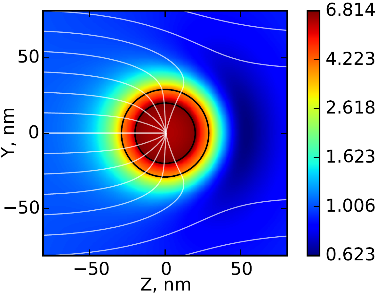
\includegraphics[width=0.99\textwidth]{3g}
  \end{minipage}%
  \caption{Absorption spectra of proposed
designs (a) and electric field-distribution in E-k (b,d,f) and H-k (c,e,g)
planes for $TiO_2$ core at  $\lambda=360$~nm
(b,c) and $\lambda=524$~nm (d,e) and Ag
core at  $\lambda=524$~nm (f,g).~
Field-distribution was calculated with Scattnlay [cite Ovidio paper]
software. \label{fig:field}}%
\end{figure}

For photocatalytic material, it is important to absorb a light
effectively on wide region of spectrum. To describe such possibility,
we analyze the integral absorption parameter (IAP)
$Q_{int} = \int Q_{abs}d\lambda$
as integration of absorption efficiency over wavelength region for
different core/shell dimensions. Fig.~\ref{fig:integral}(a,b) shows IAP versus
core/shell dimensions for the $TiO_2$
core and the Ag core, respectively.  Maximum of the IAP values for the
$TiO_2$
core is 638~nm for particle with core radius of 12~nm and shell
thickness of 52~nm and for the Ag core is 384~nm with core radius of
10~nm and shell thickness of 38~nm.

Spectrum parameters comparison for both structures is presented in Table
1. Ag core structure has two times larger $Q_{abs}$ value at the peak but 3
times smaller FWHM parameter comparing to $TiO_2$ core.


\begin{figure}[!h]
  \begin{minipage}[h]{0.47\textwidth}
    \begin{flushleft}
      a)
    \end{flushleft}
  \end{minipage}
  \begin{minipage}[h]{0.47\textwidth}
    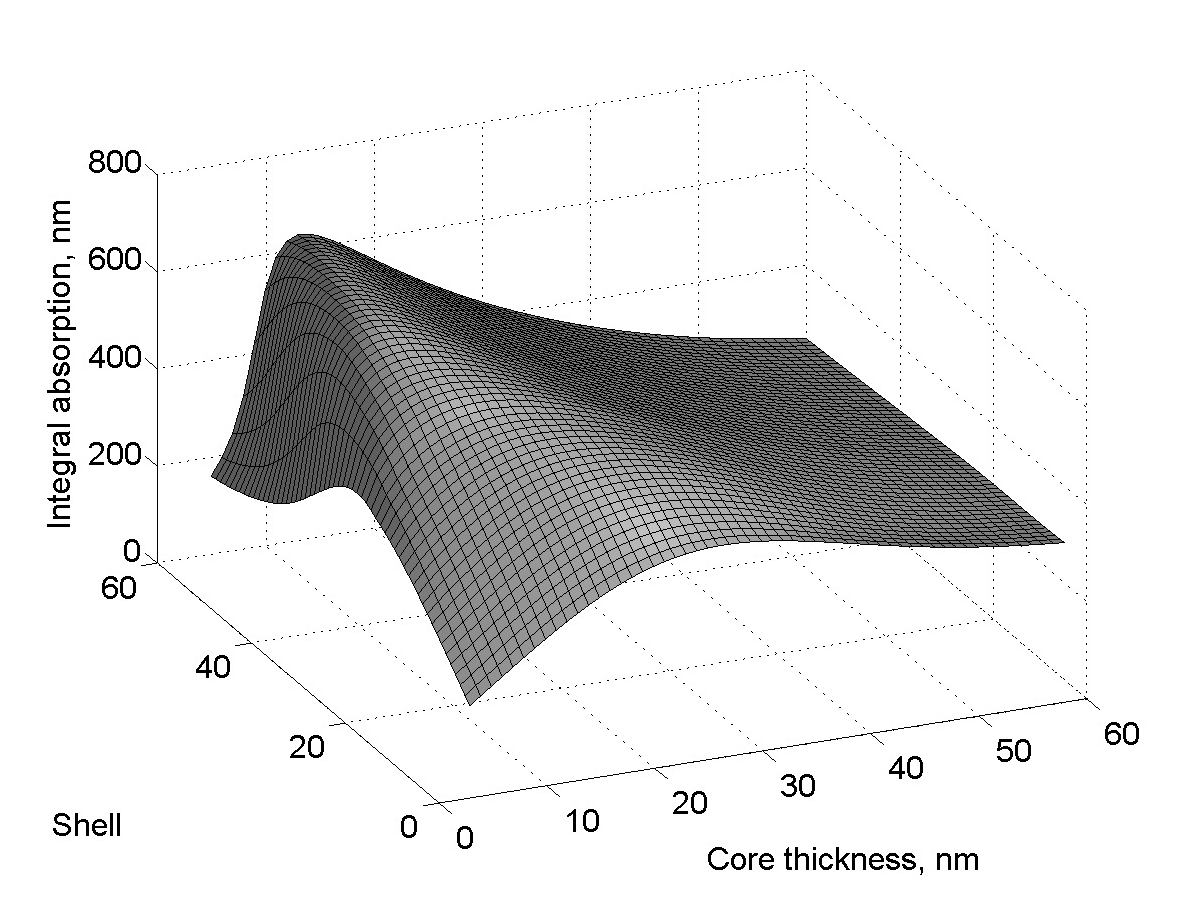
\includegraphics[width=0.99\textwidth]{Cint_TiO_Ag}
  \end{minipage}\\
  \vspace{4pt}
  \begin{minipage}[h]{0.47\textwidth}
    \begin{flushleft}
      b)
    \end{flushleft}
  \end{minipage}
  \begin{minipage}[h]{0.47\textwidth}
    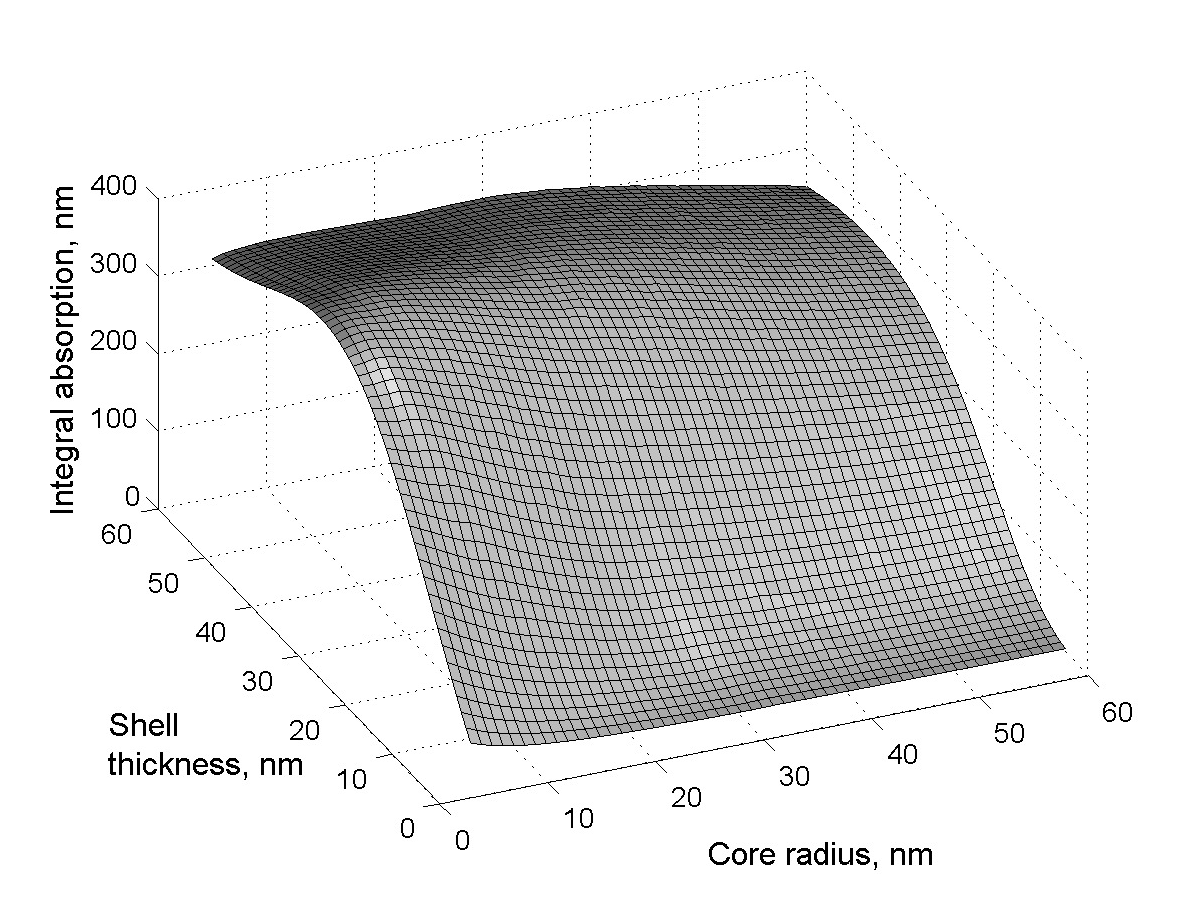
\includegraphics[width=0.99\textwidth]{Cint_Ag_TiO}
  \end{minipage}\\
  \vspace{4pt}
  \begin{minipage}[h]{0.47\textwidth}
    \begin{flushleft}
      c)
    \end{flushleft}
  \end{minipage}
  \begin{minipage}[h]{0.47\textwidth}
    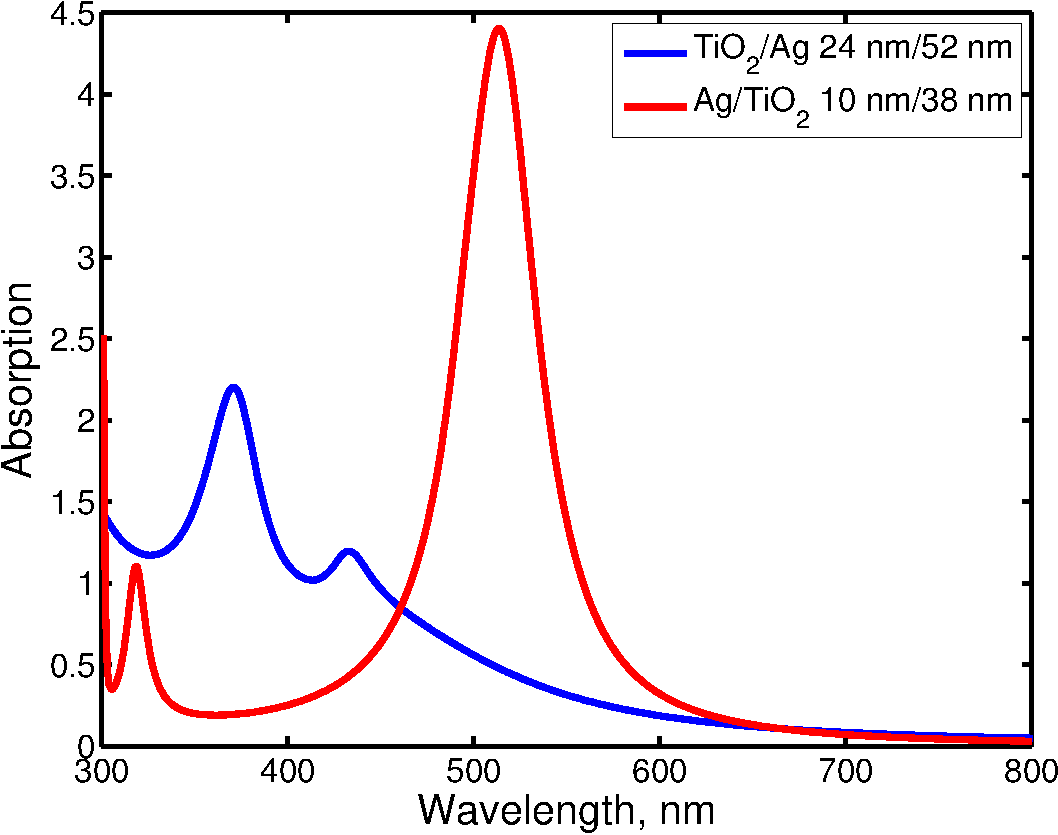
\includegraphics[width=0.99\textwidth]{compar}
  \end{minipage}%
  \caption{IAP for different core/shell
dimensions of a) $TiO_2$ core; b) Ag core; c) absorption spectra
comparison for both structures with maximum of the IAP.\label{fig:integral}}%
\end{figure}

Table 1. Comparison of spectrum parameters for $TiO_2$ core and Ag core
presented in Fig.~\ref{fig:integral}

\begin{flushleft}
\tablehead{}
\begin{supertabular}{|m{1.2191598in}|m{1.2191598in}|m{1.2191598in}|m{1.2191598in}|m{1.2198598in}|}
\hline
Structure &
the highest IAP value,~nm &
 $\text{Warning: No StarMath annotation}$ at peak,~nm &
$Q_{abs}$ at peak &
FWHM,~nm\\\hline
$TiO_2$ core &
638 &
351 &
2.21 &
141\\\hline
Ag core &
384 &
514 &
4.4 &
51\\\hline
\end{supertabular}
\end{flushleft}
Conclusion

In this paper, we compared absorption properties of $TiO_2/Ag$ and $Ag/TiO_2$
coated nanoparticle with different core/shell dimensions using Mie
scattering theory. We show the particle with core radius of 12~nm and
shell thickness of 51~nm has largest integral absorption parameter of
638~nm. Such particle can be used as effective photocatalytic material
for energy conversion applications.

References

P. Sudhagar, T.S. Song, A. Devadoss, J. W. Lee, M. H. Remon, C.
Terashima, V. V. Lysak, J. Bisquert, A. Fujishima, S. Gimenez and U.G.
Paik, Modulating the interaction between gold and $TiO_2$ nanowires for
enhanced solar driven photoelectrocatalytic hydrogen generation,
Physical Chemistry Chemical Physics, vol.17, 19371-19378, 2015

Miguel Pelaez,~Nicholas T. Nolan,~Suresh C. Pillai,~Michael K.
Seery,~Polycarpos Falaras, Athanassios G. Kontos,~Patrick S.M.
Dunlop,~Jeremy W.J. Hamilton,~J.Anthony Byrne,~Kevin
O'Shea, Mohammad H. Entezari,~Dionysios D. Dionysiou,
A review on the visible light active titanium dioxide photocatalysts
for environmental applications Applied Catalysis B: Environmental
Volume 125, 21 August 2012, Pages 331{}--349

Miguel Pelaez,~Nicholas
T. Nolan,~Suresh C. Pillai,~Michael K. Seery,~Polycarpos Falaras,
Athanassios G. Kontos,~Patrick S.M. Dunlop,~Jeremy W.J.
Hamilton,~J.Anthony Byrne,~Kevin O'Shea, Mohammad H.
Entezari,~Dionysios D. Dionysiou, A review on the visible light active
titanium dioxide photocatalysts for environmental applications Applied
Catalysis B: Environmental Volume 125, 21 August 2012, Pages 331--349

Lin H. Size dependency of nanocrystalline $TiO_2$ on its optical property
and photocatalytic reactivity exemplified by 2-chlorophenol. Appl Catal
B Environ. 2006; 68(1):1-- 11.
Etacheri V,. di Valentin C., Schneider J., Bahnemann D., Pillai S.C.
Visible light activation of $TiO_2$ photocatalyst: Advanced in theory and
experimients. J. of photochemistry and photobiology C: photochemistry
reviews 2015 25  1-29.
G. Mie, Annalen der Physik, 1908, 330, 377--445.
Rivero PJ, Goicoechea J, Urrutia A, Matias IR, Arregui FJ. Multicolor
Layer-by-Layer films using weak polyelectrolyte assisted synthesis of
Core/Shell Nanoparticles. Nanoscale Research Letters. 2013; 8:438.
Ghaforyan H, Ebrahimzadeh M, Ghaffary T, Rezazadeh H, Sokout Jahromi Z.
Microwave absorbing properties of Ni nanowires grown in nanoporous
anodic alumina templates. Chin J Phys. 2014; 52(1):233--8.
Mohammadi BS, Ebrahimzadeh M, Ghaforyan H. Simulation of optical
characteristics of nickel and nickel/ titanium dioxide. World Appl
Program. 2015; 5(7):109--12.
Ghaforyan H, Ebrahimzadeh M, Mohammadi BS. Study of the optical
properties of nanoparticles using Mie theory. World Appl Program. 2015;
5(4):79--82.
Matzler C. MATLAB functions for Mie scattering and absorption. Technical
report, Research Report No. 2002-- 08. Institute of Applied Physics,
University of Bern. 2002; 8:5--7.
U. Kreibig and M. Vollmer, Optical Properties of Metal Clusters,
Springer, New York, 1995, p. 159. 
A. D. Rakic {\textasciiacute}, A. B. Djuris \textlatin{[2C7?]}ic
{\textasciiacute}, J. M. Elazar and M. L. Majewski, Appl. Opt., 1998,
37, 5271--5283.
van de Hulst H.C. {\textquotedblleft}Light Scattering by Small
Particles{\textquotedblright}, (1957), reprinted by Dover Publication,
New York, NY (1981).
M. I. Tribelsky, EPL (Europhysics Letters), 2011, 94, 14004.
C. F. Bohren and D. Huffman, Absorption and scattering of light by small
particles, Wiley, 1983


\end{document}